\documentclass{TDP003mall}
\usepackage{graphicx}



\newcommand{\version}{Version 1.1}
\author{Jesper Skoglund, \url{jessk378@student.liu.se}\\
  Niklas Nilsson, \url{nikni292@student.liu.se}}
\title{Användarmanual}
\date{2014-09-08}
\rhead{Jesper Skoglund\\
Niklas Nilsson}



\begin{document}
\projectpage
\section{Revisionshistorik}
\begin{table}[!h]
\begin{tabularx}{\linewidth}{|l|X|l|}
\hline
Ver. & Revisionsbeskrivning & Datum \\\hline
1.0 & Första versionen skapad i latex & 150911 \\\hline
1.1 & Infogade bilder och refererade till dem & 150915 \\\hline
\end{tabularx}
\end{table}


\section{Startsidan}
Detta är den första sidan som visas när man besöker portfolion. Sidan tar upp ca 80\% av bredden på sidan och innehåller en sidfot och ett sidhuvud. 
Dessa är genomgående för alla sidor framöver. \\
Till vänster presenteras prersentatören med en text och en bild, denna information ändrar man i en JSON fil och läses in. Till höger ca 20\% av bredden 
så visas det senaste projektet kortfattat och en länk leder till dess projektsida där man kan läsa mera. \\
Se bild 1.2.

\subsection{Sidhuvud}
Sidhuvudet innehåller till vänster namn och efternman på presentatören, denna information hämtas dynamiskt via config filen. Till höger finns följande länkar: \\

1. Start - Som leder till denna sida 

2. Projekt - Som leder till en sida med alla projekt listade.
 
3. Sök - Tar dig till en söksida där man kan söka på de olika projekten. \\
Se bild 1.1.

\subsection{Sidfot}
Sidfoten innehåller till vänster kontakt information så som epost, telefonnummer och länkar till github, twitter och linkedin. Till höger finns information om skapare och versionsnummer av systemet. Information till vänster hämtas dynamiskt via config filen. \\
Se bild 1.1.

\section{Listsidan}
Denna sida visar alla projekt som har skapatas. Varje projekt visas i en <div></div> tagg som tar upp 40\% av bredden, i denna så visas projektets 
namn, tekniker och en bild. Även kortfattad beskrivning visas. Hela taggen är klickbar och leder till projektsidan där man kanb läsa mera.\\
Se bild 1.3.

\subsection{Projektsidan}
Denna sida visar projektet mer detaljerat. Till vänster finns en bild från projktet. Viktiga fält i början är \\

1. Projektets namn 

2. Datum och namn på skapare

3. Tekniker som använts 

4. Länk till github

5. Löpande text om projektet, denna text kan innehålla html taggar så som <h2> och <b>, man kan även inkludera bild och film (via andra tjänster).\\
Se bild 1.2.

\subsection{Tekniksida}
Denna sida använder man för att söka bland projekt eller se projekt som använder en viss typ av tekniker. Sidans viktiga funktioner är

1. Sök ruta som är stor och tydlig och en knapp till höger som utför sökningen. 

2. Kryssrutor för att välja tekniker, tekniken som står till höger om rutan är länkbar och visar då alla projekt med denna teknik. 

3. Sökresultat visas i samma typ av <div></div> taggar som på listsidan.\\
Se bild 1.3.
 
\clearpage

\begin{figure}[ht!]
\centering
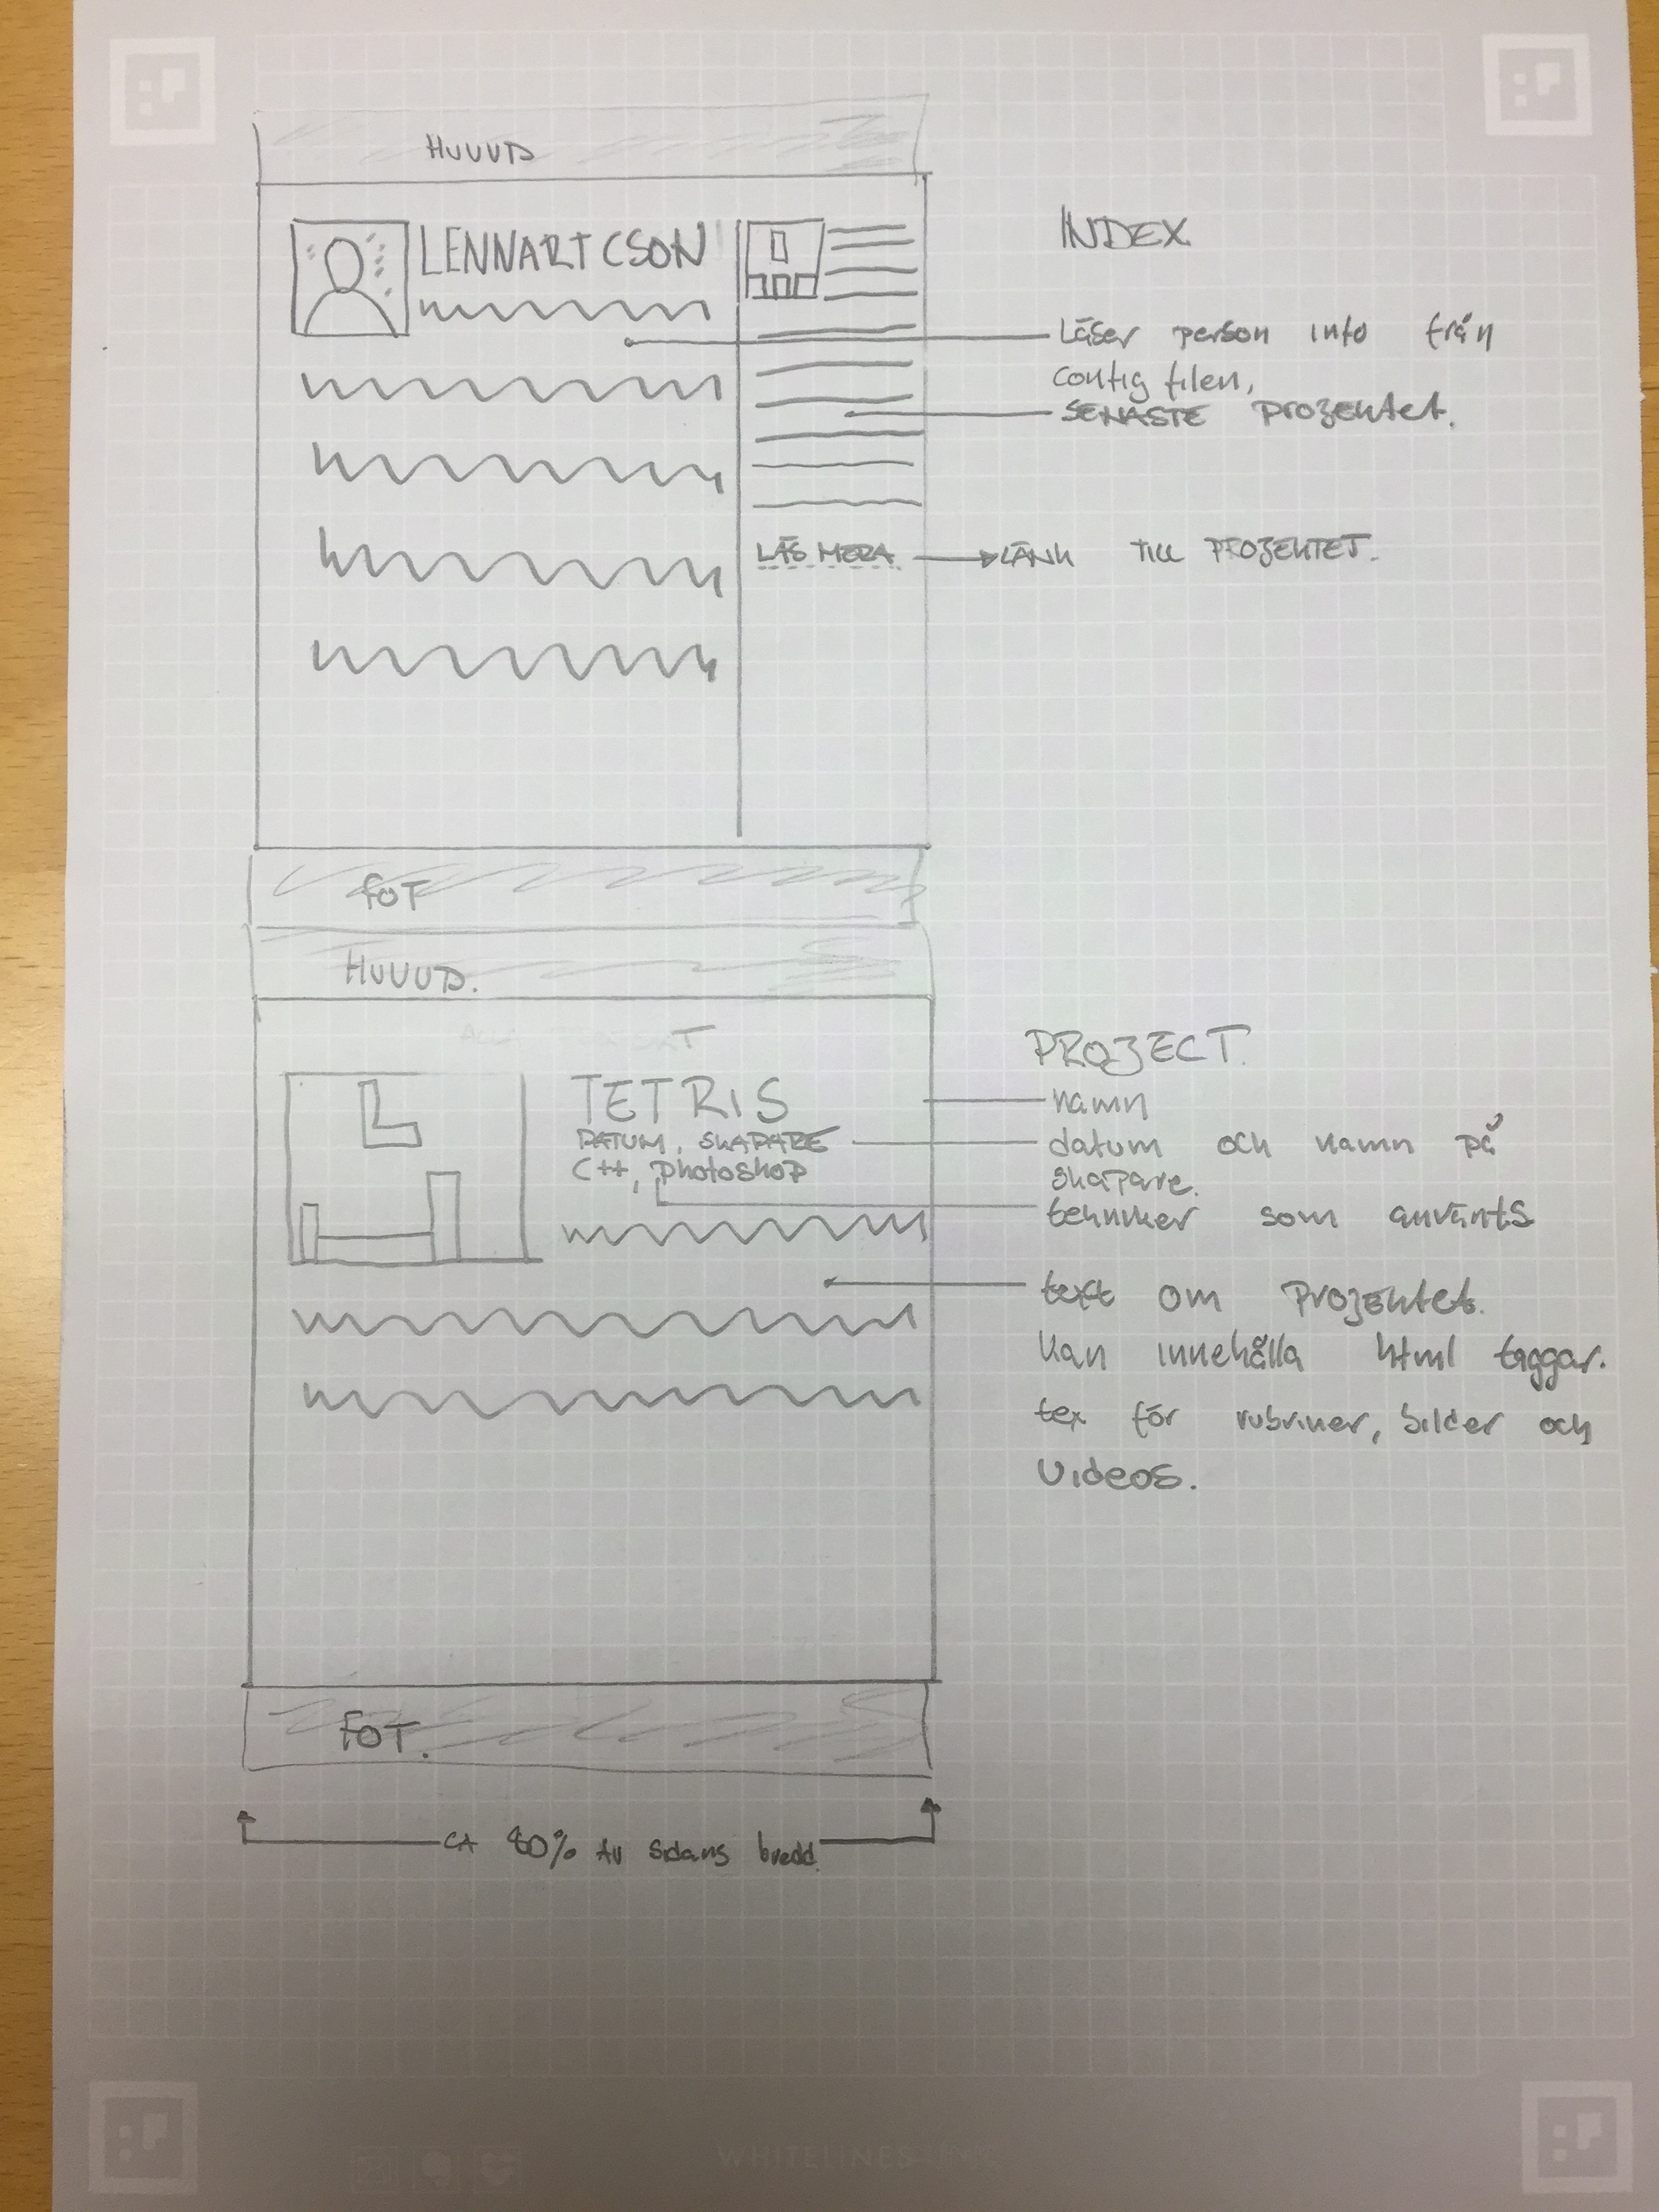
\includegraphics[width=90mm]{IMG_0065.jpg}
\caption{1.2 översikts bild projektsida och startsida} \label{start_pro}
\end{figure}

\begin{figure}[ht!]
\centering
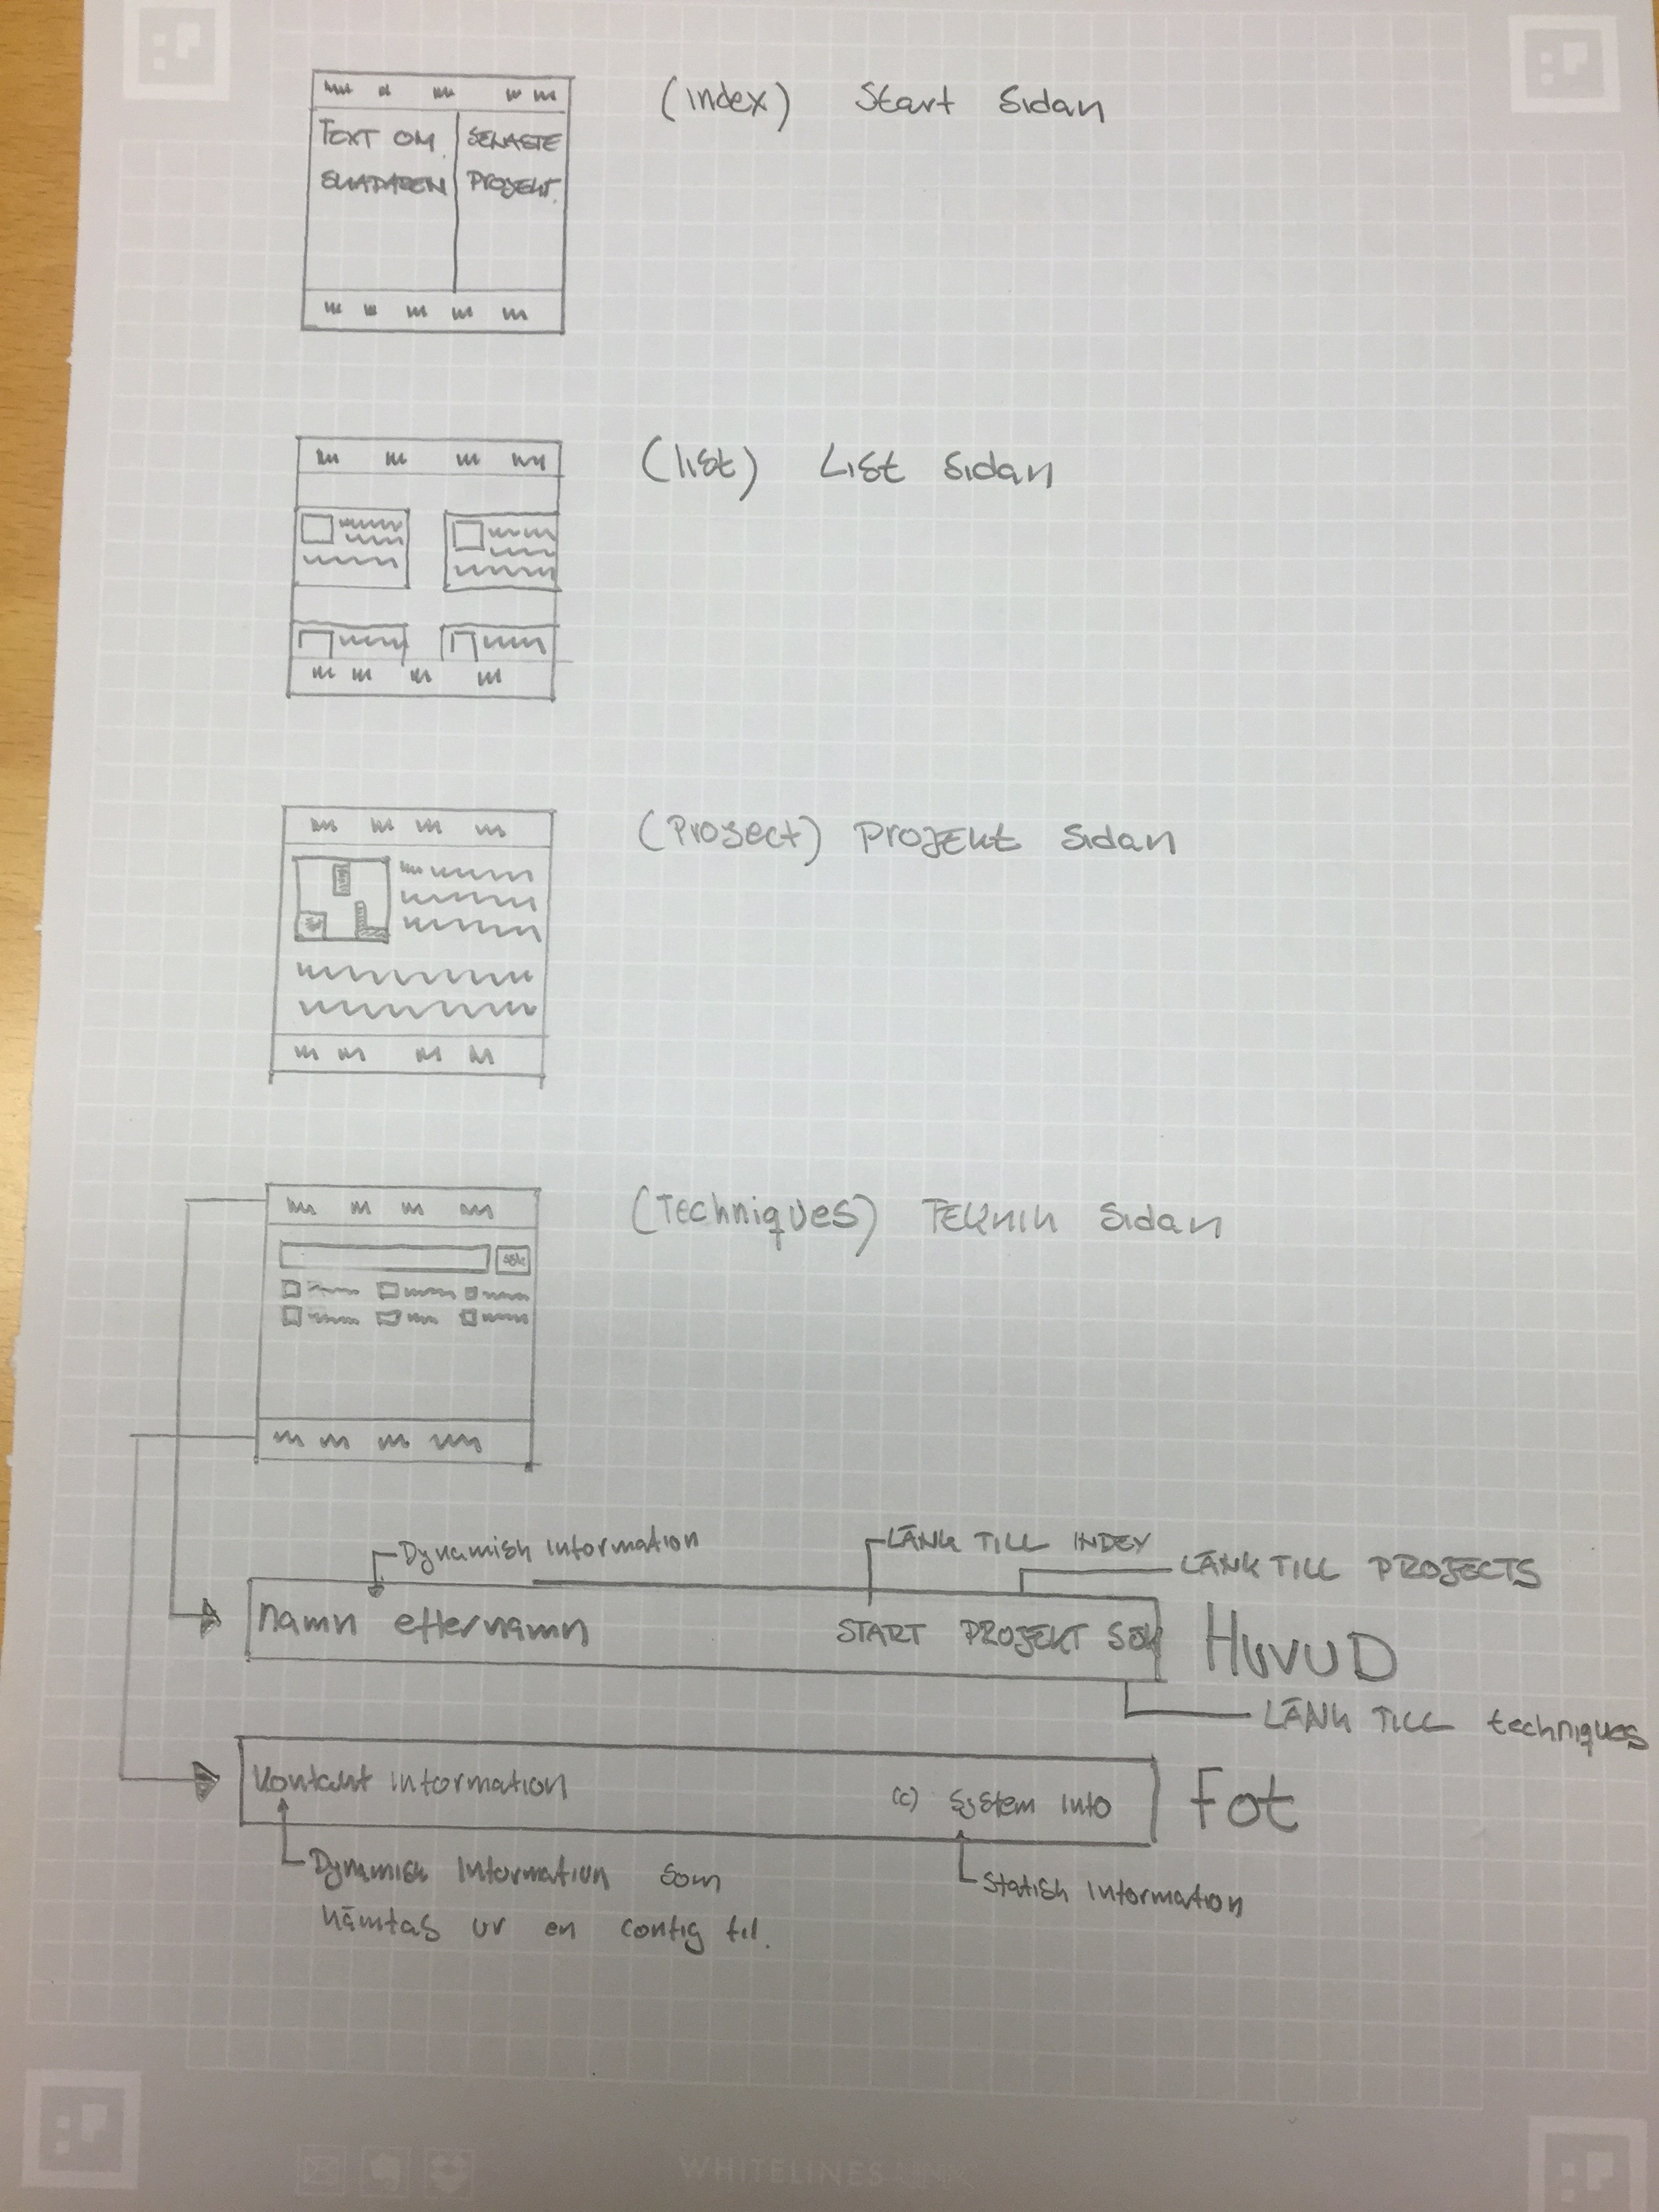
\includegraphics[width=90mm]{IMG_0062.jpg}
\caption{1.1 översikts bild på header och footer} \label{oversight}
\end{figure}

\begin{figure}[ht!]
\centering
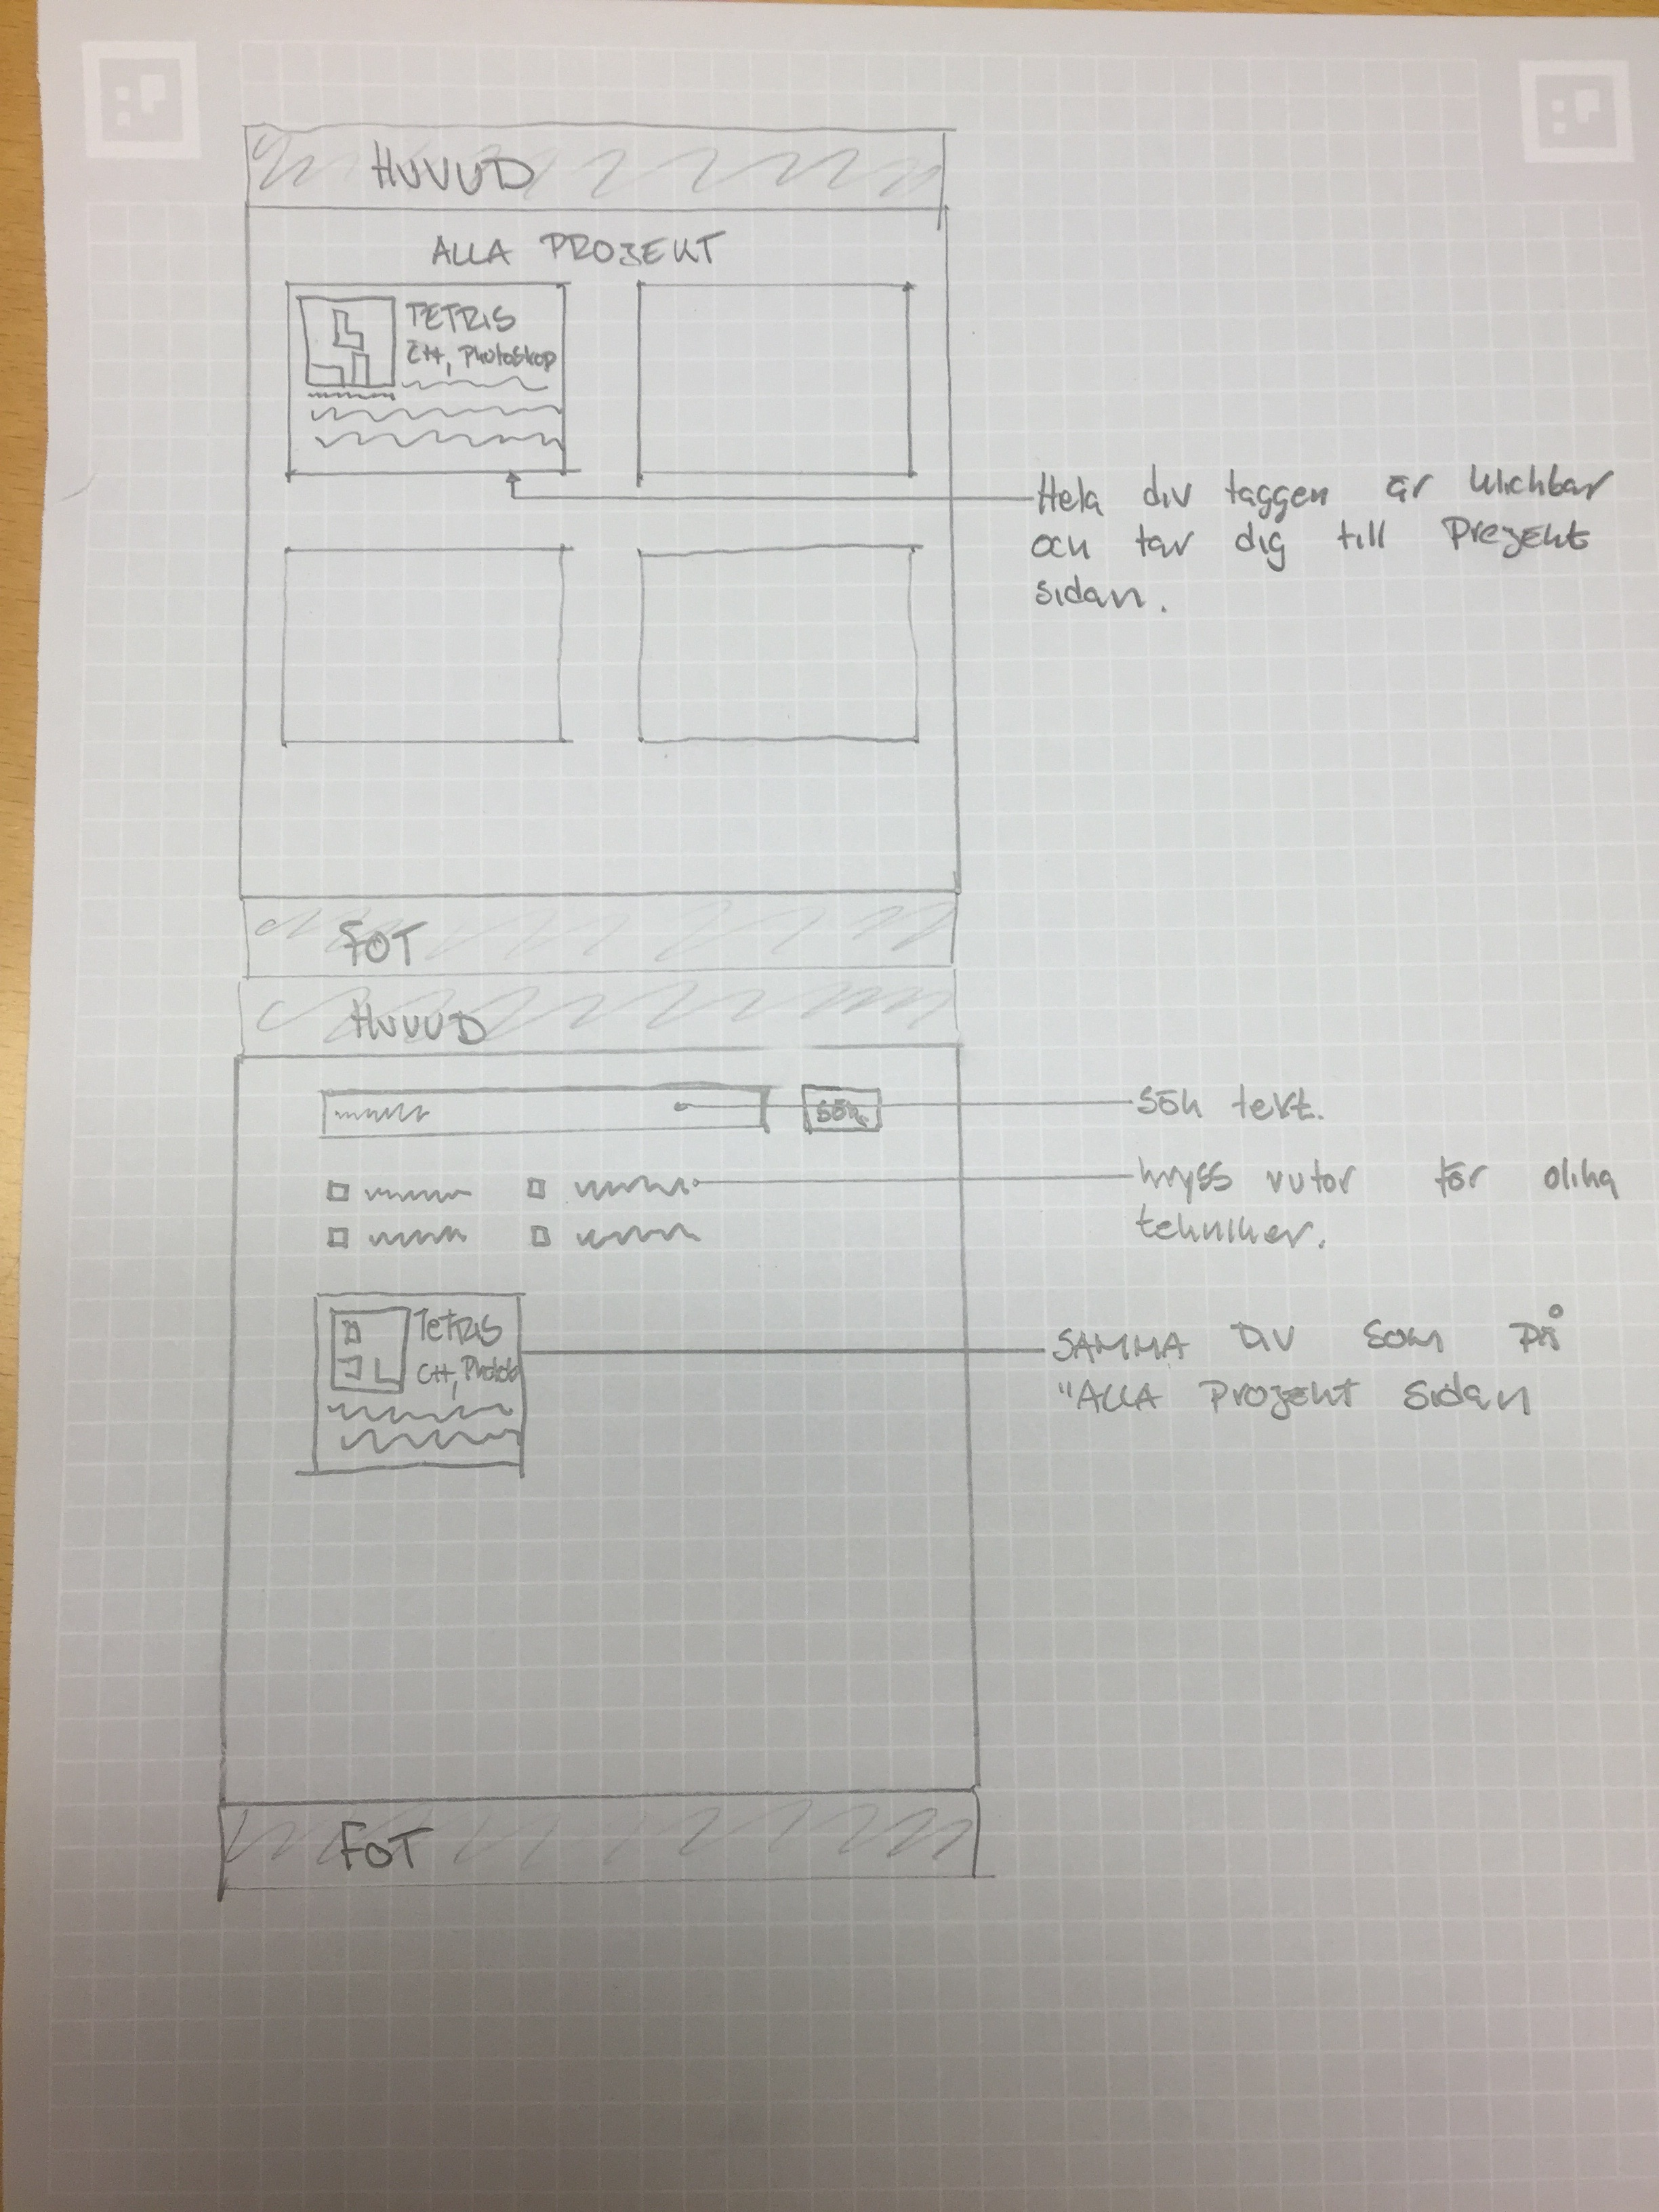
\includegraphics[width=90mm]{IMG_0066.jpg}
\caption{1.3 översikts bild på alla projekt och söksida} \label{search_all}
\end{figure}



\ref{oversight}
\ref{start_pro}
\ref{search_all}

\end{document}
